\begin{appendices}
\section{Annexes}

\subsection{Messages robot-superviseur}
\label{sec:sec:comm_rob_sup}

La communication fonctionne sur le principe d'une communication synchrone de type requête. La communication ne peut être initiée que par le superviseur.

Toutes les communications ont par défaut un retour en cas d'erreur. Ce retour est porté par la valeur de {\tt messageID} d'un objet {\tt Message}. Si la communication s'est bien déroulée la valeur MESSAGE\_ANSWER\_ACK est retournée, sinon une valeur de retour correspondante à l'un des cas d'erreur suivant est produite : 
\begin{itemize}
	\item MESSAGE\_ANSWER\_ROBOT\_TIMEOUT : la réponse n'est pas arrivée avant 80 ms,
	\item MESSAGE\_ANSWER\_ROBOT\_UNKNOWN\_COMMAND : la commande n'a pas été comprise par le robot,
	\item MESSAGE\_ANSWER\_ROBOT\_ERROR : la commande n'est pas conforme à sa définition.
\end{itemize}
\FloatBarrier

Les messages envoyés au robot sont composés d'une entête codée sur un octect ({\tt char}) correspondant à l'ordre à réaliser. Certains ordres sont aussi accompagnés d'une donnée codée sur un entier ({\tt int}). Le tableau~\ref{tab:ordre_robot} décrit les entêtes.

\begin{table}[htp]
\begin{center}
\begin{tabular}{|l|c|l|c|c|}
\hline
Entête (\scriptsize{MESSAGE\_ROBOT\_}) & Données & Description & Retour\\
\hline\hline
{\scriptsize PING} & -- & Teste la disponibilité de la communication &  --\\
{\scriptsize RESET} & -- & Demande un redémarrage du robot &  --\\
\hline
{\scriptsize START\_WITHOUT\_WD} & -- & Démarre le robot sans le {\it watchdog} & -- \\
{\scriptsize START\_WITH\_WD} &  -- & Démarre le robot avec le {\it watchdog} & -- \\
{\scriptsize RELOAD\_WD} & -- & Recharge le {\it watchdog} & --\\
\hline
{\scriptsize BATTERY\_GET} & -- & Retourne le niveau de la batterie & niv. batterie\\
{\scriptsize STATE\_GET} & -- & Retourne l'état du robot & état\\
\hline
{\scriptsize GO\_FORWARD} & -- & Déplace le robot en avant & -- \\
{\scriptsize GO\_BACK}  & -- & Déplace le robot en arrière & -- \\
{\scriptsize GO\_LEFT} & -- & Fait tourner dans le sens anti-horaire & -- \\
{\scriptsize GO\_RIGHT} & -- & Fait tourner dans le sens horaire & -- \\
{\scriptsize STOP\_MOVE} & -- & Stoppe le mouvement du robot & -- \\
\hline
{\scriptsize MOVE} & distance & Déplace en ligne droite & --\\
{\scriptsize TURN} & angle & Tourne d'un angle donné & -- \\
\hline
\end{tabular}
\end{center}
\caption{Liste des messages du superviseur vers le robot}
\label{tab:ordre_robot}
\end{table}%
\FloatBarrier

Le niveau de la batterie peut prendre comme valeur :
\begin{itemize}
	\item BATTERY\_UNKNOWN : la mesure n'a pas abouti,
	\item BATTERY\_EMPTY : niveau vide,
	\item BATTERY\_LOW : niveau faible,
	\item BATTERY\_FULL: niveau haut.
\end{itemize}

Les états possibles du robot sont :
\begin{itemize}
	\item MESSAGE\_ROBOT\_STATE\_BUSY : le robot est en train de réaliser un mouvement,
	\item MESSAGE\_ROBOT\_STATE\_NOT\_BUSY : le robot ne réalise pas de mouvement.
\end{itemize}

%%%%%%%%%%%%%%%

\subsection{Messages moniteur-superviseur}
\label{sec:comm_mon_sup}

\subsubsection{Moniteur vers Superviseur}
\label{sec:mts}

Les message envoyés du moniteur vers le superviseur sont composés d'un entête de trois octets et d'une donnée d'un octet. Le tableau~\ref{tab:mts} décrit ces entêtes et les données. Certains messages nécessitent une réponse par un acquittement (cf. messages section~\ref{sec:stm}). Les messages spécifiques pour le robot ont les même entêtes que la communication entre le robot et le superviseur.


\begin{table}[htp]

\begin{center}
\begin{tabular}{|l|p{7cm}|}
\hline
{\bf Id} & {\bf Description} \\
\hline
MESSAGE\_ROBOT\_COM\_OPEN & Demande d'ouverture de la comm. avec le robot\\
MESSAGE\_ROBOT\_COM\_CLOSE  & Demande de fermeture de la comm. avec le robot \\
\hline
\multicolumn{2}{|l|}{{\bf Acquittement} : oui}\\
\hline
\hline
MESSAGE\_ROBOT\_* & Message portant un ordre pour le robot (voir tableau précédent)\\
\hline
\multicolumn{2}{|p{\textwidth}|}{{\bf Acquittement} : les messages MESSAGE\_ROBOT\_START\_WITH\_WD et MESSAGE\_ROBOT\_START\_WITHOUT\_WD nécessitent un acquitement}\\
\hline
\hline
MESSAGE\_CAM\_OPEN & Demande d'ouverture de la caméra\\
MESSAGE\_CAM\_CLOSE  & Demande de fermeture de la caméra\\
MESSAGE\_CAM\_ASK\_ARENA  & Demande de détection de l'arène \\
MESSAGE\_CAM\_ARENA\_CONFIRM  & L'arène est la bonne\\
MESSAGE\_CAM\_ARENA\_INFIRM  & L'arène n'est pas la bonne\\
MESSAGE\_CAM\_POSITION\_COMPUTE\_START  & Calcul de la position du robot\\
MESSAGE\_CAM\_POSITION\_COMPUTE\_STOP  & Arrêt du calcul de la position du robot\\
\hline
\multicolumn{2}{|p{\textwidth}|}{{\bf Acquittement} : les messages MESSAGE\_CAM\_OPEN et  MESSAGE\_CAM\_CLOSE attendent un acquittement.}\\
\hline
\end{tabular}
\end{center}
\caption{Description des messages du moniteur vers le superviseur}
\label{tab:mts}
\end{table}%

\newpage
%%%%%%%%%
\subsubsection{Superviseur vers Moniteur}
\label{sec:stm}

Les messages du superviseur vers le moniteur sont composés d'une entête de 3 octets et de données de taille variables. Le tableau~\ref{tab:stm} décrit ces messages.

\begin{table}[htp]
\begin{center}
\begin{tabular}{lcl}
\hline
Entête & Données & Description\\
\hline
\hline
MESSAGE\_ANSWER\_ACK & -- & Message d'acquittement en cas de succès\\
MESSAGE\_ANSWER\_NACK & -- & Message d'acquittement en cas d'échec\\
MESSAGE\_MONITOR\_LOST  & -- & Signale la perte de la comm. avec le robot\\
MESSAGE\_CAM\_IMAGE  & Image & Envoi d'une image\\
MESSAGE\_CAM\_POSITION & Position & Envoi de la postion du robot\\
MESSAGE\_ROBOT\_BATTERY\_LEVEL  & int & Envoi du niveau de la batterie\\
\hline
\end{tabular}
\end{center}
\caption{Liste des messages du moniteur vers le superviseur}
\label{tab:stm}
\end{table}%
\FloatBarrier

\newpage
\section{Diagramme de classe des bibliothèques}
\label{ann:diag_class}

%
%@startuml
%skinparam monochrome true
%
%class Message{
%-MessageID messageID
%
%+Message()
%+Message(MessageId id)
%+string ToString()
%+bool CompareID(MessageID id)
%+MessageID GetID()
%+void SetID(MessageID id)
%-bool CheckID(MessageID id)
%}
%
%
%class MessageBattery{
%    -BatteryLevel level
%    +MessageBattery(MessageID id, BatteryLevel level)
%    +BatteryLevel GetLevel()
%    +void SetLevel(BatteryLevel level)
%}
%
%class MessagePosition{
%    -Position pos
%    +MessagePosition(MessageID id, Position& pos)
%    +Position GetPosition()
%    +void SetPosition(Position& pos)
%}
%
%class MessageImg{
%    -Img* image
%    +MessageImg(MessageID id, Img *image)
%    +Img* GetImage()
%    +void SetImage(Img* image)
%}
%
%class MessageInt{
%    - int value
%    + MessageInt(MessageID id, int val)
%    +int GetValue()
%    +void SetValue(int val)
%}
%
%class MessageString{
%    - string s
%    +MessageString(MessageID id, string s)
%    +string GetString()
%    +void SetString(string s)
%}
%
%Message <|-down- MessageImg
%Message <|-down- MessageInt
%Message <|-up- MessageString
%Message <|-up- MessageBattery
%Message <|-- MessagePosition
%
%class ComRobot {
%  +int Open()
%  +int Open(string usart)
%  +int Close()
%  +Message *Write(Message* msg)
%  +void Write_Pre()
%  +void Write_Post()
%  +Message *Ping()
%  +Message *Reset()
%  +Message *PowerOff()
%  +Message *StartWithWD()
%  +Message *StartWithoutWD()
%  +Message *ReloadWD()
%  +Message *Move(int length)
%  +Message *Turn(int angle)
%  +Message *Stop()
%  +Message *GoForward()
%  +Message *GoBackward()
%  +Message *GoLeft()
%  +Message *GoRight()
%  +Message *GetBattery()
%  +Message *GetState()
%}
%
%class ComMonitor {
%  +int Open(int port)
%  +void Close()
%  +int AcceptClient()
%  +void Write(Message *msg)
%  +void Write_Pre()
%  +void Write_Post()
%  +Message *Read()
%  +void Read_Pre()
%  +void Read_Post()
%}
%class Img{
%    +ImageMat img
%    +Img(ImageMat imgMatrice)
%    +string ToString()
%    +Jpg ToJpg()
%    +Arena SearchArena()
%    +int DrawRobot(Position robot)
%    +int DrawArena(Arena arenaToDraw)
%    +std::list<Position> SearchRobot(Arena arena)
%}
%
%class Camera{
%    +Camera(int size, int fps);
%
%    +bool Open();
%    +void Close();
%    +Img Grab();
%    +int GetWidth() const;
%    +int GetHeight() const;
%
%    +bool IsOpen();
%    +void SetSize(int size);
%}
%
%class Position{
%    +cv::Point2f center
%    +cv::Point2f direction
%    +float angle
%    +int robotId
%}
%
%class Arena{
%    +cv::Rect arena
%    +Arena()
%    +bool IsEmpty()
%}
%
%@enduml

 \begin{figure}[htbp]
\begin{center}
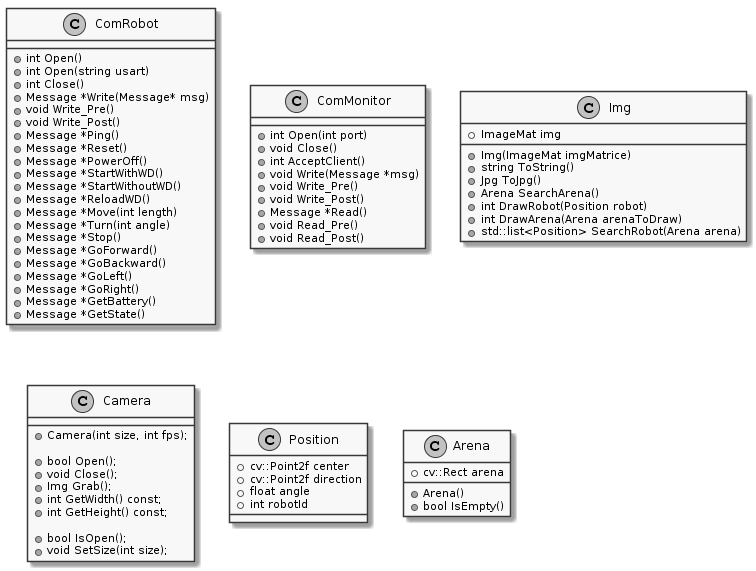
\includegraphics[scale=0.55]{./figures_pdf/classes1}
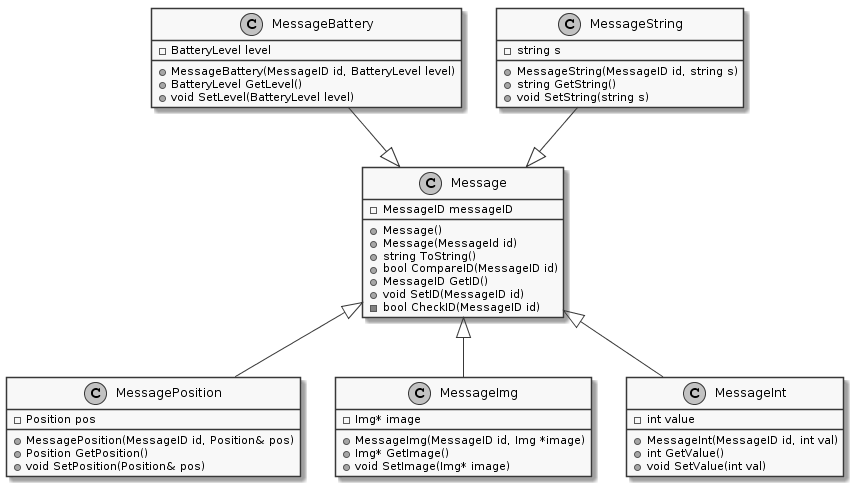
\includegraphics[scale=0.55]{./figures_pdf/classes2}
\caption{Diagramme de classes des bibliothèques De Stijl}
\label{fig:diag17}
\end{center}
\end{figure}
\FloatBarrier
\end{appendices}